\section{Simulation with Proteus}
It is a good practice to simulate a circuit before connecting it, in order to avoid hardware damage/debug issues in a circuit beforehand. We used \emph{Proteus Professional} 8 for this purpose. Proteus has libraries for most commonly used electronics components, and it also allows us to make our own components, thanks to which we could download unavailable components from the internet, where many users have shared their own custom components.
\begin{figure}[H]
	\vfill
	\centering
	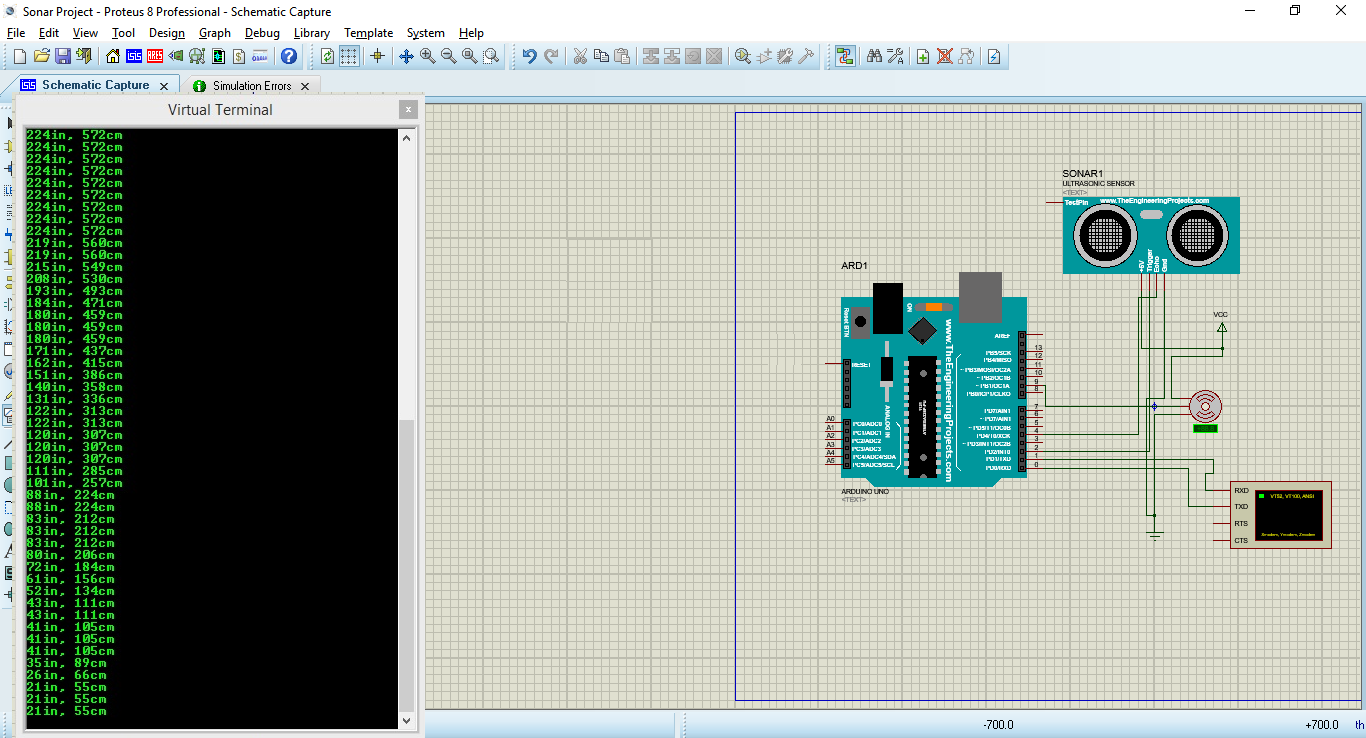
\includegraphics[width=0.7\textwidth]{../Files/proteus}
	\caption{The Proteus Simulator}  \label{fig:proteus}
\end{figure}

\section{Processing}
Processing is an interactive software to write programs with visual output. We have used Processing 3.2 for generating a 2D radar-map representation of the serial data being obtained from the Arduino through the computer's serial port.
\begin{figure}[H]
	\vfill
	\centering
	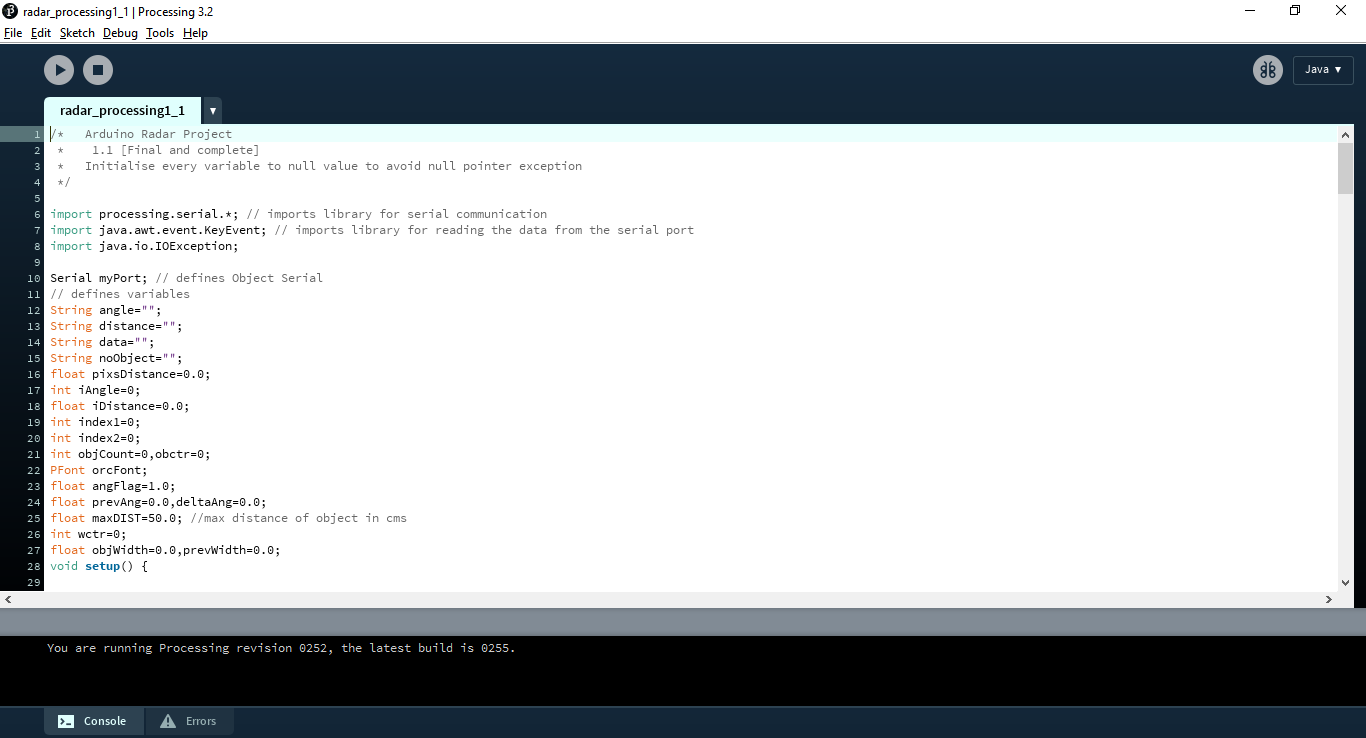
\includegraphics[width=0.7\textwidth]{../Files/processing}
	\caption{Processing}  \label{fig:processing}
\end{figure}
The code in Processing is written in \emph{Java}, and primarily consists of drawing the lines and borders of the radar map, and plotting the tracker-bar on the map. We added functionalities such as counting the number of objects, and also tried to calculate the width of the object, apart from just showing the distance of the object. \\
We made a 360 degrees map so that we could view the area according to our convenience if the angle of the set-up is changed. This angle is the "offset" that we introduced in the Arduino code. The entire Arduino and Processing codes are shown in Appendix \ref{ch:appAlabel} and Appendix \ref{ch:appBlabel}, respectively.
\begin{figure}[H]
	\vfill
	\centering
	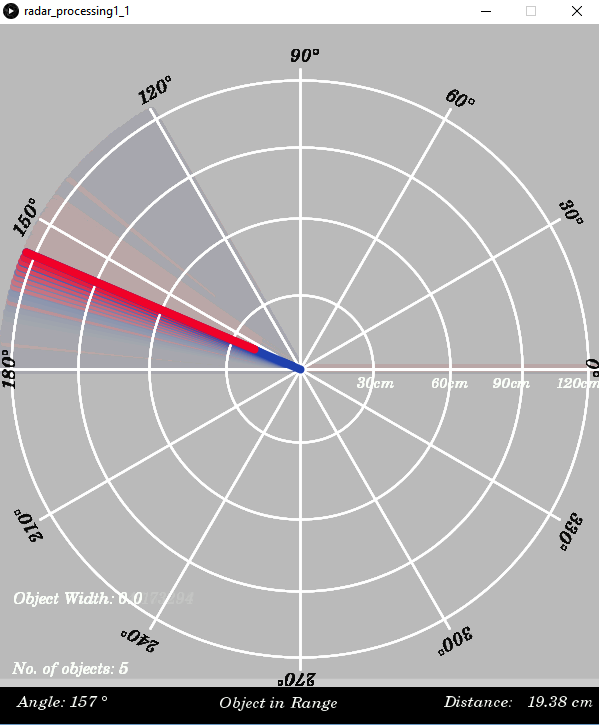
\includegraphics[width=0.7\textwidth]{../Files/radar}
	\caption{Running our code in Processing}  \label{fig:radar}
\end{figure}
\clearpage